% !TEX root = ../main.tex

\section{Основні поняття теорії ймовірностей}
\subsection{Теоретико-множинний підхід до основних понять ТЙ}
\begin{definition}
    \emph{Стохастичним експериментом (випробуванням)} називається експеримент, 
    який можна повторювати неодноразово, зберігаючи певні умови, і результат якого 
    експерименту заздалегідь передбачити неможливо.
\end{definition}
\begin{definition}
    Будь-який результат СЕ називається \emph{подією}.
\end{definition}
\begin{example}
    \begin{enumerate}
        \item СЕ --- кидання кубика один раз, подія --- випало 6 очок.
        \item СЕ --- кидання кубика двічі, подія --- сума очок, що випала, дорівнює 6.
    \end{enumerate}
\end{example}

\noindent \textbf{Події бувають:}
\begin{enumerate}
    \item Випадкові --- можуть відбутися чи не відбутися при проведенні СЕ.
    \item Неможливі --- ніколи не відбуваються в даному СЕ.
    \item Вірогідні --- завжди відбуваються в даному СЕ.
\end{enumerate}

Будемо вважати, що кожному СЕ можна поставити у відповідність деяку множину, що
називається \emph{простором елементарних подій} $\Omega$. 
Під \emph{елементарними подіями} $\omega$ будемо розуміти єдині
логічно можливі події СЕ, що виключають одна одну.
\begin{example}
    \begin{enumerate}
        \item СЕ --- кидання кубика один раз. 
        $\Omega = \left\{\omega_1, \omega_2, ..., \omega_6\right\}$, 
        де події 

        $\omega_k = \left\{\text{випало } k \text{ очок}\right\}, k = 1,...,6$.
        \item СЕ --- кидання монетки до першої появи герба.
        $\Omega = \left\{\omega_1, \omega_2, ..., \omega_k, ...\right\}$, 
        
        де $\omega_i = \left\{\text{герб випав на }i\text{-тому киданні}\right\}, i\in \mathbb{N}$.
        \item СЕ --- зустріч двох осіб, що домовилися зустрітися протягом години.
        $x$ --- час приходу першої особи, $y$ --- час приходу другої, $0\leq x, y \leq 1$.
        $\Omega = \left\{ \left( x, y\right): 0\leq x, y \leq 1\right\}\subset \mathbb{R}^2$.
    \end{enumerate}
\end{example}
В подальшому випадкові події позначатимемо $A, B, C, ...$. 
\emph{Випадкова подія --- підмножина $\Omega$}. 
У прикладі з киданням кубика один раз $A = \left\{\text{випало }6\text{ очок}\right\} = \left\{ \omega_6\right\}$.
В загальному випадку маємо $A = \left\{\omega_{k1}, \omega_{k2}, ..., \omega_{kn}, ...\right\} \subset \Omega$.
Неможлива подія --- $\varnothing$, вірогідна --- $\Omega$. 

\begin{remark}
    Розглядаємо події в межах фіксованих СЕ та простору елементарних подій.
\end{remark}
\begin{enumerate}
    \item \emph{Включення} $A \subset B$ означає, що якщо відбулася подія $A$, то обов'язково відбудеться подія $B$.
    Наприклад, $A = \left\{\text{витягнуто даму пік}\right\}, B = \left\{\text{витягнуто карту чорної масті}\right\}$. 
    Очевидно, $A\subset B$.

    Рівність подій: $\left( A \subset B, B \subset A \right) \iff \left( A = B\right)$.
    \item \emph{Об'єднання подій} $A \cup B$ --- це подія, яка відбувається тоді, коли відбувається
    принаймні одна з подій $A$ чи $B$.

    Властивості: $A \cup A = A$,  $A \cup B = B \cup A$, $\left( A \subset B \right) \Rightarrow \left( A \cup B = B \right)$, 
    $A \cup \Omega = \Omega$, $A \cup \varnothing = A$, $\left( A \cup B \right) \cup C = A \cup \left( B \cup C \right)$.

    Операція узагальнюється на скінченну або зліченну кількість подій: $A = \bigcup\limits_{i=1}^{n \left( \infty \right)} A_i$.
    \item \emph{Перетин подій} $A \cap B$ --- це подія, яка відбувається тоді, коли $A$ і $B$ відбуваються одночасно.

    Властивості: $A \cap A = A$,  $A \cap B = B \cap A$, $\left( A \subset B \right) \Rightarrow \left( A \cap B = A \right)$, 
    $A \cap \Omega = A$, $A \cap \varnothing = \varnothing$, $\left( A \cap B \right) \cap C = A \cap \left( B \cap C \right)$,
    $A \cap B \subset A$, $A \cap B \subset B$, $\left( A \cup B \right) \cap C = \left( A \cap C \right) \cup \left( B \cap C \right)$,
    $\left( A \cap B \right) \cup C = \left( A \cup C \right) \cap \left( B \cup C \right)$.

    Операція узагальнюється на скінченну або зліченну кількість подій: $A = \bigcap\limits_{i=1}^{n \left( \infty \right)} A_i$.
\end{enumerate}
\begin{definition}
    Події $A$ та $B$ називається \emph{несумісними}, якщо вони не відбуваються одночасно: $A \cap B = \varnothing$.
    Узагальнення: події $A_1, A_2, ..., A_n, ...$ називаються \emph{попарно несумісними}, якщо $A_i \cap A_j = \varnothing$ для $i \neq j$.
\end{definition}
\begin{definition}
    Події $A_1, A_2, ..., A_n, ...$ утворюють \emph{повну групу подій}, якщо вони попарно несумісні 
    та $\bigcup\limits_{i=1}^{n \left( \infty \right)} A_i = \Omega$.
\end{definition}
\begin{enumerate}
    \setcounter{enumi}{3}
    \item \emph{Протилежна подія} $\overline{A}$ --- це подія, яка відбувається тоді, коли $A$ не відбувається.
    
    Властивості: $A \cup \overline{A} = \Omega$, $A \cap \overline{A} = \varnothing$, $\overline{\left( A \cup B \right)} = \overline{A} \cap \overline{B}$,
    $\overline{\left( A \cap B \right)} = \overline{A} \cup \overline{B}$.
    \item \emph{Різниця подій} $A \backslash B$ --- це подія $A \cap \overline{B}$. Для протилежної події маємо $\overline{A} =  \Omega \backslash A$.
\end{enumerate}

\begin{definition}
    Непорожня система підмножин $\mathcal{F}$ простору елементарних подій $\Omega$ утворює \emph{алгебру подій}, якщо:
    \begin{enumerate}
        \item $\Omega \in \mathcal{F}$;
        \item $\left( A, B \in \mathcal{F}\right) \Rightarrow \left( A \cup B \in \mathcal{F}\right)$;
        \item $\left( A \in \mathcal{F}\right) \Rightarrow \left( \overline{A} \in \mathcal{F}\right)$.
    \end{enumerate}
    \emph{Узагальнення:} якщо $\Omega$ містить зліченну кількість подій, то означення $\sigma$-алгебра отримаємо заміною умови
    2 на $\left(\forall n \in \mathbb{N}: A_n \in \mathcal{F} \right) \Rightarrow \left( \bigcup\limits_{n=1}^{\infty} A_n \in \mathcal{F}\right)$.
    
    Пара $\left\{\Omega, \mathcal{F}\right\}$ називається \emph{вимірним простором стохастичного експерименту}.
\end{definition}

\subsection{Класична модель ймовірності}
Дослідника завжди цікавить кількісна характеристика появи тієї чи іншої події.

Нехай $\Omega$ --- скінченний чи зліченний. 
Поставимо у відповідність кожній елементарній події $\omega_k$ число $p_k\geq 0$ так, що $\sum\limits_{k=0}^{ n \left( \infty\right)}p_k = 1$.
Тоді $P(A) = \sum\limits_{\omega_k \in A} p_k$ --- кількісна характеристика, ймовірність події $A$.

\begin{example}
    \emph{Класична модель ймовірності}. Якщо простір елементарних подій $\Omega$ СЕ скінченний
    та всі $\omega_k$ рівноможливі, то такий СЕ називається \emph{класичним}.
    В такому випадку $p_1 = p_2 = ... = p_n = \frac{1}{n}$, де $n = \mathrm{card}(\Omega)$.
    
    \begin{equation}\label{eq:m_n}
        P(A) = \sum\limits_{\omega_k \in A} p_k = \frac{m}{n} = \frac{\text{кількість елементарних подій в } A}{\text{загальна кількість елементарних подій}}
    \end{equation}
\end{example}
Ймовірності, що розраховуються за формулою \eqref{eq:m_n}, називаються \emph{класичними}.
\begin{example}
    \begin{enumerate}
        \item <<Задачі про вибір>> --- коли з великої кількості чогось вибирають певну кількість.
        Наприклад, з урни з 10 кульками, 3 чорними та 7 білими, навмання витягають 5 кульок.
        Обчислимо ймовірність події $A = \left\{ \text{серед них 2 чорних кульки}\right\}$:
        $P(A) = \frac{C_3^2\cdot C_7^3}{C_{10}^5} = \frac{3\cdot 35}{252} = \frac{5}{12}$.
        \item <<Задачі про ліфт>>. 5 осіб одночасно зайшли в ліфт 11-поверхового будинку. 
        Яка ймовірність того, що вони всі вийдуть на різних поверхах, починаючи з другого?
        
        $P(A) = \frac{A_{10}^5}{\widetilde{A}_{10}^5} = \frac{10\cdot 9\cdot 8\cdot 7 \cdot 6}{10^5} = 0.3024$. 
        Тут $A_n^k$ та $\widetilde{A}_n^k$ --- кількості розміщень без повторень та з повтореннями відповідно.
    \end{enumerate}
\end{example}

\noindent \textbf{Властивості класичної ймовірності:}
\begin{enumerate}
    \item $\forall A \in \mathcal{F}: 0 \leq P(A) \leq 1$.
    \item $P(\Omega) = 1$.
    \item $P(\overline{A}) = 1 - P(A)$.
    \item $P(\varnothing) = 0$.
    \item $P(A\cup B) = P(A) + P(B) - P(A\cap B)$, для несумісних $A$ і $B$ $P(A\cup B) = P(A) + P(B)$.
    \item $\left( A \subset B\right) \Rightarrow \left( P(A) \leq P(B)\right)$.
    \item Якщо $A_1, A_2, ..., A_n$ --- повна група подій СЕ, то $P\left(\bigcup\limits_{i=1}^{n} A_i\right) = 1$.
\end{enumerate}

\subsection{Геометрична модель ймовірності}
\begin{example}
    Нехай точка кидається навмання на відрізок $\left[a; b\right]$. 
    Яка ймовірність її 
    потрапляння в $\left<\alpha; \beta\right> \subset  \left[a; b\right]$?
    Розглянемо подію $A = \left\{ 
        \text{точка потрапила в} \left<\alpha; \beta\right>
    \right\}$.
    \newline
    \hbox to \hsize{\hfil{
        \begin{tikzpicture}
            \draw [fill] (0, 0) circle [radius = 0.05];
            \node [below] at (0, 0) {$a$};
            \node [above] at (0, 0) { };
            \node [below] at (8, 0) {$b$};
            \draw [-{Straight Barb}] (6,0) to (2,0) {};
            \draw [-{Straight Barb}] (2,0) to (6,0) {};
            \node [below] at (2, 0) {$\alpha$};
            \node [below] at (6, 0) {$\beta$};
            \draw [fill] (8, 0) circle [radius = 0.05];
            \draw [thick] (0, 0) -- (8, 0);
        \end{tikzpicture}
    }\hfil}
    Логічно припустити, що $P(A) = k\cdot l_{\left<\alpha; \beta\right>}$ для деякого $k > 0$.
    Тоді $P(\Omega) = 1 = k\cdot l_{\left[a; b\right]}$. Таким чином, 
    $k = \frac{1}{l_{\left[a; b\right]}} = \frac{1}{b-a}$,
    тому $P(A) = \frac{l_{\left<\alpha; \beta\right>}}{l_{\left[a; b\right]}}$.
\end{example}
Нехай простір елементарних подій інтерпретується як замкнена область в 
$ \mathbb{R} ^n$, а випадкові події --- її підмножини. В якості $\sigma$-алгебри 
подій $\mathcal{F}$ беремо підмножини, що мають міру $\mu$. Тоді в якості ймовірності 
деякої події $A$ беремо $P(A) = \frac{\mu(A)}{\mu(\Omega)}$. 
Наприклад, в $\mathbb{R}^1$ беремо міру <<довжина>>, в $\mathbb{R}^2$ --- <<площа>>, а в $\mathbb{R}^3$ --- <<об'єм>>.

Ймовірності, що знаходяться таким чином називаються \emph{геометричними}, а сама модель 
називається \emph{геометричною моделлю ймовірності}.
Геометрична модель може використовуватись, 
коли $\Omega$ має геометричну інтерпретацію як замкнена область в $\mathbb{R}^n$,
а елементарні події --- рівноможливі.

\begin{example}[задача Бюффона]\label{buffon}
    На площині накреслені паралельні прямі на відстані $2a$, на них кидається 
    голка довжиною $2l,\; l \leq a $. Яка ймовірність того, що голка перетне 
    яку-небудь пряму?
    \newline
    \hbox to \hsize{\hfil{
        \begin{tikzpicture}[scale = 0.5]
            \draw [thick] (0, 0) -- (8, 0);
            \draw [thick] (0, 2) -- (8, 2);
            \draw [thick] (0, 4) -- (8, 4);
            \draw [thick] (0, 6) -- (8, 6);
            \draw [{Straight Barb}-{Straight Barb}] (7.5,4) to (7.5,6);
            \node [right] at (7.5, 5) {$2a$}; 
        \end{tikzpicture}
        \begin{tikzpicture}[scale = 1]
            \draw (0, 0) -- (4, 0);
            \draw (0, 2) -- (4, 2);
            \draw [thick] (0.5, -0.5)-- (2.5, 1.5);
            \draw [{Straight Barb}-{Straight Barb}] (3.5,0) to (3.5,2);
            \draw [{Straight Barb}-{Straight Barb}] (1.5,0) to (1.5,0.5);
            \node [right] at (3.5, 1) {$2a$};
            \node [right] at (1.5, 0.25) {$ x $};
            \draw [-{Straight Barb}](2.5, 0) to [out = 90, in = 0](1.75, 0.75);
            \node [right] at (2.28, 0.53) {$ \varphi $};
        \end{tikzpicture}
    }\hfil}
    Достатньо розглядати лише дві прямі. $\Omega = \left\{(\varphi, x)\in 
    \mathbb{R}^2: \varphi \in \left[0; \pi\right], x \in \left[0; a\right] 
    \right\}$
    \newline
    При такій побудові простору елементарних подій подія $A = \left\{\text{голка 
    перетне пряму}\right\} =$
    \newline
    $\left\{(\varphi, x)\in 
    \Omega: x\leq l\sin\varphi\right\}$
    \newline
    \hbox to \hsize{\hfil{
        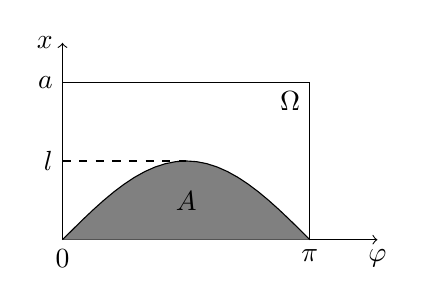
\begin{tikzpicture}
            \draw [<->] (4, 0) -- (0, 0) -- (0, 2.5);
            \node [left] at (0, 2.5) {$x$};
            \node [below] at (4, 0) {$\varphi$};
            \draw [domain=0:pi,fill=gray] plot (\x, {1*sin(\x r)});
            \node [below] at (0, 0) {$0$};
            \node [below] at (pi, 0) {$\pi$};
            \draw [dashed] (0,1) to (pi/2,1);
            \node [left] at (0, 1) {$l$};
            \draw (0,2) -- (pi, 2) -- (pi, 0);
            \node [left] at (0, 2) {$a$};
            \node [below left] at (pi, 2) {$\Omega$};
            \node [above] at (pi/2, 0.25) {$A$};
        \end{tikzpicture}
    }\hfil}
    $P(A) = \frac{S(A)}{S(\Omega)},\; S(\Omega) = \pi a,\;S(A) = \int\limits_0^\pi 
    l\sin\varphi\ d\varphi = l\left.(-\cos\varphi)\right|^\pi_0 = 2l$.
    Отже, $P(A) = \frac{2l}{\pi a}$.
    \newline
    Якщо провести $n$ кидань голки, у $m$ з яких голка потрапить на пряму, то за допомогою приблизної рівності $\frac{m}{n} 
    \approx \frac{2l}{\pi a}$ можна приблизно обчислити число $\pi$. 
    Наприклад, якщо взяти $n=5000, m=2532, l/a = 0.8$, то отримаємо $\pi \approx 3.1596$.
\end{example}
\begin{example}[парадокс Бертрана]
    Нехай в колі радіусом $R$ навмання обирається хорда. Яка ймовірність того, 
    що її довжина буде більшою за довжину сторони правильного трикутника, 
    вписаного в це коло?
    \newline
    Існують три способи розв'язання цієї задачі, причому кожен з них дає різний результат.
    
    \textbf{Спосіб 1.}
    З міркувань симетрії обирається якийсь фіксований діаметр кола і розглядається
    всі перпендикулярні до нього хорди. Серед них і обирається навмання довільна хорда.
    Очевидно, що кожна хорда у цьому випадку може бути однозначно визначена своєю серединою,
    тобто кожній хорді можна взаємно однозначно поставити у відповідність координату її середини,
    якщо за початок відліку взяти якийсь з кінців фіксованого діаметру.
    \newline
    \hbox to \hsize{\hfil{
        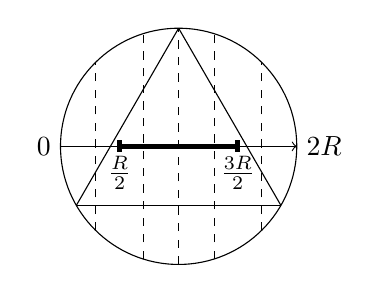
\begin{tikzpicture}[scale = 1.5]
            \draw (0, 0) circle [radius = 1]; 
            \draw (0, 1) -- (-0.86602540378, -0.5); 
            \draw (0, 1) -- (0.86602540378, -0.5);
            \draw (0.86602540378, -0.5) -- (-0.86602540378, -0.5);
            \draw [->] (-1,0) to (1, 0);
            \node [left] at (-1, 0) {$0$};
            \node [right] at (1, 0) {$2R$};
            \draw [dashed] (0, -1) to (0, 1);
            \draw [dashed] (-0.3, -0.954) to (-0.3, 0.954);
            \draw [dashed] (-0.7, -0.714) to (-0.7, 0.714);
            \draw [dashed] (0.3, -0.954) to (0.3, 0.954);
            \draw [dashed] (0.7, -0.714) to (0.7, 0.714);
            \draw [ultra thick] (-0.5, 0) -- (0.5, 0);
            \draw [ultra thick] (-0.5, 0.05) -- (-0.5, -0.05);
            \draw [ultra thick] (0.5, 0.05) -- (0.5, -0.05);
            \node [below] at (-0.5, 0) {$\frac{R}{2}$};
            \node [below] at (0.5, 0) {$\frac{3R}{2}$};
        \end{tikzpicture}
    }\hfil}
    Таким чином, множина всіх значень координати середини хорди $\Omega = \left[0; 2R\right]$. 
    Множина, що відповідає події --- це відрізок $A = \left[\frac{R}{2}; \frac{3R}{2}\right]$.
    В якості міри візьмемо довжину. Тоді $P(A) = \frac{l(A)}{l(\Omega)} = \frac{R}{2R}= \frac{1}{2}$.
    
    \textbf{Спосіб 2.}
    В цьому способі пропонується розглядати тільки хорди з одним закріпленим кінцем.
    Кожній хорді поставимо у відповідність ту частину дуги кола, яка потрапляє у кут $\varphi$,
    що утворює хорда з дотичною, проведеною через точку закріплення кінця всіх хорд.
    \newline
    \hbox to \hsize{\hfil{
        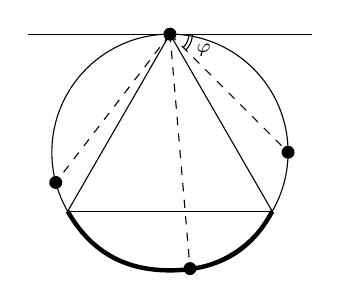
\begin{tikzpicture}[scale = 1.5]
            \draw (0, 0) circle [radius = 1];
            \draw (0, 1) -- (-0.86602540378, -0.5); 
            \draw (0, 1) -- (0.86602540378, -0.5);
            \draw (0.86602540378, -0.5) -- (-0.86602540378, -0.5);
            \draw (-1.2, 1) -- (1.2, 1);
            \draw [fill] (0, 1) circle [radius = 0.05];
            \draw [fill] (0.17, -0.985) circle [radius = 0.05];
            \draw [fill] (1, 0) circle [radius = 0.05];
            \draw [fill] (-0.967, -0.256) circle [radius = 0.05];
            \draw (0.16, 1) arc (0:-46:0.16);
            \draw (0.19, 1) arc (0:-46:0.19);
            %\node [above] at (0, 1);
            \draw [dashed] (0, 1) to (0.17, -0.985);
            \draw [dashed] (0, 1) to (1, 0);
            \draw [dashed] (0, 1) to (-0.967, -0.256);
            \node [below right] at (0.14, 1) {$_\varphi$};
            \draw [ultra thick](0.86602540378, -0.5) to [out = 242, in = 0](0, -1);
            \draw [ultra thick](0, -1) to [out = 180, in = 300](-0.86602540378, -0.5);
        \end{tikzpicture}
    }\hfil}
    Тоді множина $\Omega = \left[ 0; \pi\right]$, а $A = \left[ \frac{\pi}{3}; \frac{2\pi}{3}\right]$.
    Знову візьмемо за міру довжину і отримаємо $P(A) = \frac{\pi /3}{\pi} = \frac{1}{3}$.
    
    \textbf{Спосіб 3.}
    Розглядаються всі хорди кола. Кожній з них взаємно однозначно ставиться у відповідність точка її середини $(x,y)$,
    якщо за початок координат прийняти центр кола.
    \newline
    \hbox to \hsize{\hfil{
        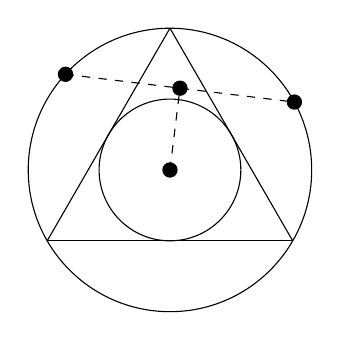
\begin{tikzpicture}[scale = 1.8]
            \draw (0, 0) circle [radius = 1];
            \draw (0, 0) circle [radius = 0.5];
            \draw (0, 0) [fill] circle [radius = 0.05];
            \draw (0, 1) -- (-0.86602540378, -0.5); 
            \draw (0, 1) -- (0.86602540378, -0.5);
            \draw (0.86602540378, -0.5) -- (-0.86602540378, -0.5);
            \draw (-0.737, 0.675) [fill] circle [radius = 0.05];
            \draw (0.878, 0.479) [fill] circle [radius = 0.05];
            \draw [dashed] (-0.737, 0.675) to (0.878, 0.479);
            \draw [dashed] (0, 0) to (0.0705, 0.577);
            \draw (0.0705, 0.577) [fill] circle [radius = 0.05];
        \end{tikzpicture}
    }\hfil}
    В такому випадку $\Omega = \left\{ (x,y)\in \mathbb{R}^2: x^2 + y^2 \leq R^2\right\}$,
    а $A = \left\{ (x,y)\in \Omega: x^2 + y^2 \leq \frac{R^2}{4}\right\}$.
    Тоді $P(A) = \frac{\pi R^2/4}{\pi R^2} = \frac{1}{4}$.

    Жозеф Бертран був противником геометричного означення ймовірності.
    Він казав, що воно не дає можливості однозначно обчислити ймовірність
    однієї і тієї ж випадкової події та використовував вищенаведений приклад
    для доведення своєї правоти. Дійсно, було отримано три різних відповіді при
    розв'язанні однієї задачі. Так в чому ж справа? Насправді, помилка полягає
    у різних трактуваннях поняття <<навмання обрана хорда>>.
    В кожному з трьох способів це трактування було різним, що й стало причиною різних відповідей.
\end{example}
